This chapter will cover background theory of technology and techniques used in this project. 
The first section, \Cref{sec:twitterapi} covers the API used to retrieve data from Twitter. In \Cref{sec:nodejs}, the Node.js platform is introduced, and in \Cref{sec:ml} different machine learning algorithms gets a short explanation. Finally in \Cref{sec:backgroundslr} the systematic literature review process is presented. 


\section{Twitter API}~\label{sec:twitterapi}
Twitter allows developers and others to access their data by the means of an application program interface (API). The API is implemented by using Representational State Transfer (REST). REST is a style of software architecture for distributing data across the World Wide Web (WWW). By using the protocol HTTP's vocabulary of methods, developers can get, insert, delete and update data on Twitter, given the proper access. Some of the important methods are GET for retrieving data, POST for inserting, updating and sending data, DELETE for removing data.~\citep{article:rest}

Twitter uses OAuth for authentication. OAuth provides a way for clients to access resources on behalf of end users or other clients. OAuth is also used to provide third party applications access to a users data on a service, without sharing the users user name or password.~\citep{site:oauth}

After migrating to version 1.1 of their API, Twitter now has a limit on the number of requests an end user can do. As end users authenticate using OAuth, Twitter can identify them and limit their access if overused. The limitations are divided into 15 minute intervals. Some services on the API are limited to 15 requests per time window, other services are limited by 180 requests. E.g. the search service is limited by 180 requests, but the service for retrieving tweets from a Twitter list is limited by 15.~\citep{site:twitterlimit}

Almost every aspect of Twitter is covered by the REST API. The most interesting parts are the ones to retrieve tweets in various ways. There are methods for retrieving entire user time-lines, mentions of a user, favourite tweets for a user, tweets based on geographical annotated locations, and so on.~\citep{site:twitterapi}

There are also real time streaming services in the API. Streams are not based on the Twitter REST API. For streaming a persistent HTTP connection is opened to the API. This way a client would not have to continuously poll the REST API to register changes or new data. A client would be provided by real time data from Twitter, but only have one single connection opened.~\citep{site:twitterstream}

The Twitter API uses JavaScript Object Notation (JSON) as their format for response. JSON is a lightweight data format often used as an alternative to XML. JSON was created by~\citeauthor{site:json} to be a subset of the JavaScript Programming Language but still be language-independent. JSON has a simple structure and aims to be minimal, portable and textual and has support for four primitive types (strings, numbers, booleans, and null) and two structure types (array and objects).~\citep{site:json}



\section{Node.js}~\label{sec:nodejs}
Node.js is a platform built on Google's V8 JavaScript Engine. In later years Node.js has grown rapidly in popularity, much due to its scalability and event driven nature. As Node.js uses a asynchronous non-blocking I/O model, it is perfect for data-intensive real-time applications~\citep{site:nodejs}. Node.js is often refereed to as JavaScript on the server-side. 

The original goal of Node.js was to enable push capabilities for web sites. That is, for servers to be able to push states to the client, without the client having requested it first. 

Since Node.js is JavaScript based and JSON is a subset of JavaScript, JSON is integrated seamlessly. 

Although Node.js is a fairly new platform, it has a rapid growing user base. Even though Node.js was conceptualized not long ago, and is not yet released as a stable version, there are about 19,000 modules released for it through the Node Package Manager (NPM)~\citep{site:npm}. There are about 700,000 module downloads each day, using NPM. 	

\section{Machine Learning}~\label{sec:ml}
The following section describes the basic ideas for the most used machine learning methods in Twitter Sentiment Analysis. These techniques are implemented in machine learning libraries for several programming languages, such as Python and Java.
	\subsection{Naive Bayes classifier}
	\subsubsection{Naive Bayes Classifier}
		The naive Bayes classifier(NBC) is a practical Bayesian learning model that are easy to understand and implement. For some classification tasks it has proven to be equally performing to more complex classifiers like artificial neural networks(ANN) and decision trees(DT)[ref]. NBC is used for learning cases where an instance $x$ consists of a number of attribute-value pairs, and the target function $f(x)$ consists of a finite number of values from a set $V$.

The NBC is based on an assumption that all the attribute values are conditionally independent given the target value of the instance.
\begin{equation}
\label{equation:nbc}
v_{NB} = P(v_j) \amalg p(a_i|v_j)
\end{equation}

To classify an instance, the classifier's using the Maximum Likelihood Estimation(MLE) method to find the ratio of an attribute value and a given target value in the same instance in the training corpus. This means that it has to calculate the probability estimate $P$ for each attribute $a_i$, given the target value. It then assigns the target value as the one that gives the highest product from multiplying all the probabilities $P$ from the training data.
	
	\subsection{Maximum Entropy}
	Maximum Entropy (MaxEnt) is a multinomial logistic regression model that allows for classification with more than two discrete classes. It has been used for various natural language tasks, such as POS tagging and text segmentation~\citep{article:nigam}.

The principle in MaxEnt is to model all that is known and assume nothing about that which is unknown. In other words, if you have some knowledge about a domain, choose a model that is consistent with the knowledge, but otherwise as uniform as possible.

The MaxEnt models are feature-based, and in binary classification scenarios it is the same as general logistic reasoning. Unlike NB it has no assumptions of conditionally independence, and can therefore be used with feature selection methods like n-grams and extended unigrams (unigrams with negation support)~\citep{article:go}.
	
	\subsection{Support Vector Machines}
	Support Vector Machines (SVM) are often called the large margin classifiers because SVM tries to separate learning data with the highest possible margin~\citep{article:fletcher}. By separating classes in the training data with a high margin, it will obtain a better accuracy when classifying unobserved instances. Basically, SVM can only classify binary problems, however by dividing the problem into several subclassifications, SVM can be used for multi-class tasks also.

\begin{figure}[ht]
	\begin{minipage}[b]{0.45\linewidth}
		\centering
		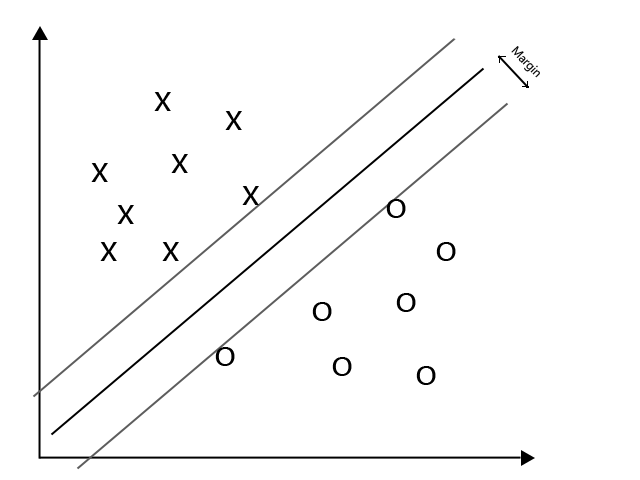
\includegraphics[width=\textwidth]{figs/linear.png}
		\caption{The hyperplane linearly separates the data into two classes. The points closest to the hyperplane are the support vectors.}
		\label{fig:linear}
	\end{minipage}
	\hspace{0.5cm}
	\begin{minipage}[b]{0.45\linewidth}
		\centering
		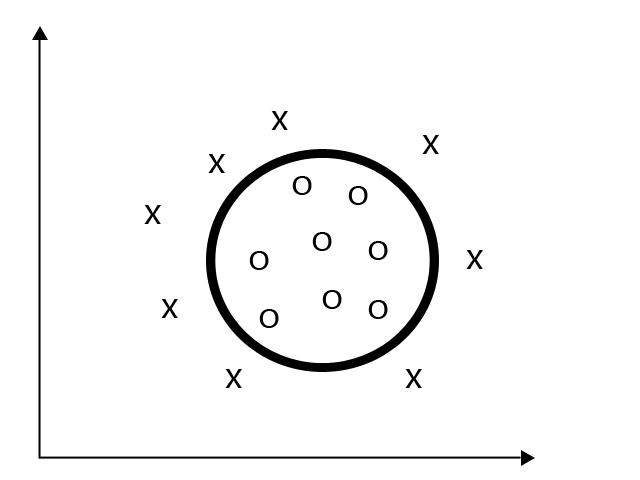
\includegraphics[width=\textwidth]{figs/non-linear.png}
		\caption{An example of a non-linear problem. A kernel function is used to map these data points into a higher dimensional feature space.}
		\label{fig:non-linear}
	\end{minipage}
\end{figure}

The equation for the separating hyperplane is defined by the closest points to the margin, as seen in~\autoref{fig:linear} These points are called \emph{support vectors}. In cases where the data is non-linear, as in~\autoref{fig:non-linear}, a kernel function is used to project the data into a high-dimensional space where it is linearly separable.


\section{Systematic Literature Review}~\label{sec:backgroundslr}
This section will describe what a systematic literature review (SLR) is and how it is conducted. 

A SLR is a methodological and formal way of retrieving information and doing literature search regarding a topic. SLR has been used to a great extent in fields like medicine, but not as much in computer science. An SLR uses several steps to accomplish the literature search and uses a systematic literature review protocol to document these steps. This way the literature search can be reproducible and is documented~\citep{paper:slrdesc}.

\subsection{Performing a SLR}

An SLR consists of three phases with 13 steps in total: planning, conducting and reporting, as defined by \cite{paper:slrdesc} and \cite{master:slr}:

\subsubsection{Planning}

\begin{description}

	\item[1. Identification of the need for a review] \hfill \\
		Identify whether or not the researchers need to review literature using SLR.

	\item[2. Commissioning a review] \hfill \\
		Organizations need to have the resources to do an SLR and commission the review.

	\item[3. Specifying the research question(s)] \hfill \\
		Define research questions (RQ) to specify what the researchers hope to find information about. The RQs are used as basis for, among others, the search, inclusion, and data collection in the conduction phase. 

	\item[4. Developing a review protocol] \hfill \\
		Develop a protocol providing documentation for all steps for conducting an SLR.
	

	\item[5. Evaluating the review protocol] \hfill \\
		Have an independent party or person evaluate the protocol.

\end{description}

% This probably shouldn't be here but in the SLR chapter..
% In this report both step 1 and 2 are assumed completed.

\subsubsection{Conducting}

\begin{description}

	\item[1. Identification of research] \hfill \\
		Locate as many papers as possible relevant to the previously defined and documented RQs. The search strategy needs to be documented with clear definitions for search domains and search string.

	\item[2. Selection of primary studies] \hfill \\
		Use a set of inclusion criteria (IC) to select what papers to use for the review. This can be done in two steps, by filtering on only title and abstract or based on the full text paper. 

	\item[3. Study quality assessment] \hfill \\
		Use a set of quality criteria (QC) to further filter down the paper collection. Use the QCs to set a score of each paper. Set a lower score limit to filter irrelevant or papers of poor quality.

	\item[4. Data extraction and monitoring] \hfill \\
		Extract data from all the papers selected and included. This data collection should be documented by the protocol, defining what features and information to extract.
	

	\item[5. Data synthesis] \hfill \\
		Synthesise the data to be able to answer the RQs. 
\end{description}

% This probably shouldn't be here but in the SLR chapter..
% For this report, the data synthesis is included as a part of the data extraction. 

\subsubsection{Reporting}


\begin{description}

	\item[1. Specifying dissemination strategy] \hfill \\
		Specify how the review result shall be presented. 

	\item[2. Formatting the main report] \hfill \\
		Report the literature review in its own report or as a part of a report.

	\item[3. Evaluating the report] \hfill \\
		Have an independent expert in the field evaluate the SLR. 

\end{description}

